\chapter{Background} \label{chapter:background}


\section{Existing Applications}

% overview

There are a number of existing applications available that attempt to solve the problem posed by this project. These range from fitness applications to various navigation applications, which although may not be completely relevant to this project, do provide some similar features such as place recognition that will be useful to research.

Table \ref{table:existing-walking-apps} shows how well each of the existing applications related to this project have implemented certain features. The maximum score for the feature category is displayed in brackets. The full matrix detailing what aspects each feature category is split into and why the score was given to each app can be seen in Appendix \ref{appendix:existing-apps-matrices}.

\begin{table}[htb]
  \centering
  \begin{tabular}{|m{2cm}||c|c|M{1.5cm}|M{1.5cm}|c|c|}
    \hline
    \textbf{Features} & \textbf{MapMyWalk} & \textbf{Strava} & \textbf{Let's Walk} & \textbf{Google Maps} & \textbf{Citymapper} & \textbf{Pok\'{e}mon Go}\\
    \hline
    \hline
    Design (2) & 1 & 2 & 0 & 2 & 2 & 2\\
    \hline
    Ease of use (3) & 3 & 3 & 1 & 3 & 3 & 3\\
    \hline
    Tracking location (2) & 2 & 2 & 2 & 1 & 1 & 1\\
    \hline
    Navigation (4) & 3 & 1 & 1 & 3 & 1 & 2\\
    \hline
    Social interaction (5) & 2 & 2 & 2 & 0 & 0 & 0\\
    \hline
    \hline
    Total (16) & 11 & 10 & 6 & 8 & 7 & 9\\
    \hline
  \end{tabular}  
  \caption{Matrix showing how well existing walking apps perform at given features. Each app is given a score for a category, with the maximum score shown in brackets next to the feature category.}
  \label{table:existing-walking-apps}
\end{table}

The rest of this section discusses each application in detail, explaining their benefits and limitations. All of the applications researched are free to use unless stated otherwise.

% go through each existing app, discussing why they are good/bad with images

\subsection{MapMyWalk}

MapMyWalk \cite{Map} is a popular fitness application for iOS and Android that allows you to track your walks and complete challenges to help you keep fit. You are able to track a walk as you go on one, or log a previous workout that you have done without the app. The app also provides a premium subscription for \pounds4.49 per month, which gives you the ability to monitor your heart rate and set training goals designed to help you walk more.

The area in which MapMyWalk lacks is social interaction. A user can publish a walk that they have previously tracked to their profile, but there is no real aspect of communication with other users other than adding each other as friends. There is also a limited level of gamification in the app, with challenges being the only option available to encourage a higher rate of fitness. Challenges can either be added by the user or chosen from a precompiled list, with the latter being fairly limited in the range of options to choose from.

\subsection{Strava}

Strava \cite{StravaInc.} is another fitness application that primarily focuses on running and cycling. It features a sleek user interface with similar functionalities as MapMyWalk. The journey view within the application can switch between either showing the map of your workout or a statistics screen as shown in Figure \ref{fig:strava}, visibly showing the time elapsed in the workout, the distance travelled and your average pace per kilometre. Strava also provides a premium subscription for \pounds5.99 per month, which features personalised coaching and advanced analysis of your workouts.

The setback of Strava is that you cannot track walks in the app as you are constrained to either running or cycling. With regards to this project, it performs well in allowing the user to record and share their workouts but it does not provide any features for the user to explore areas around them. This is expected given that it is a fitness application and does not cater for walking whatsoever.

\begin{figure}[hbt]
  \centering
  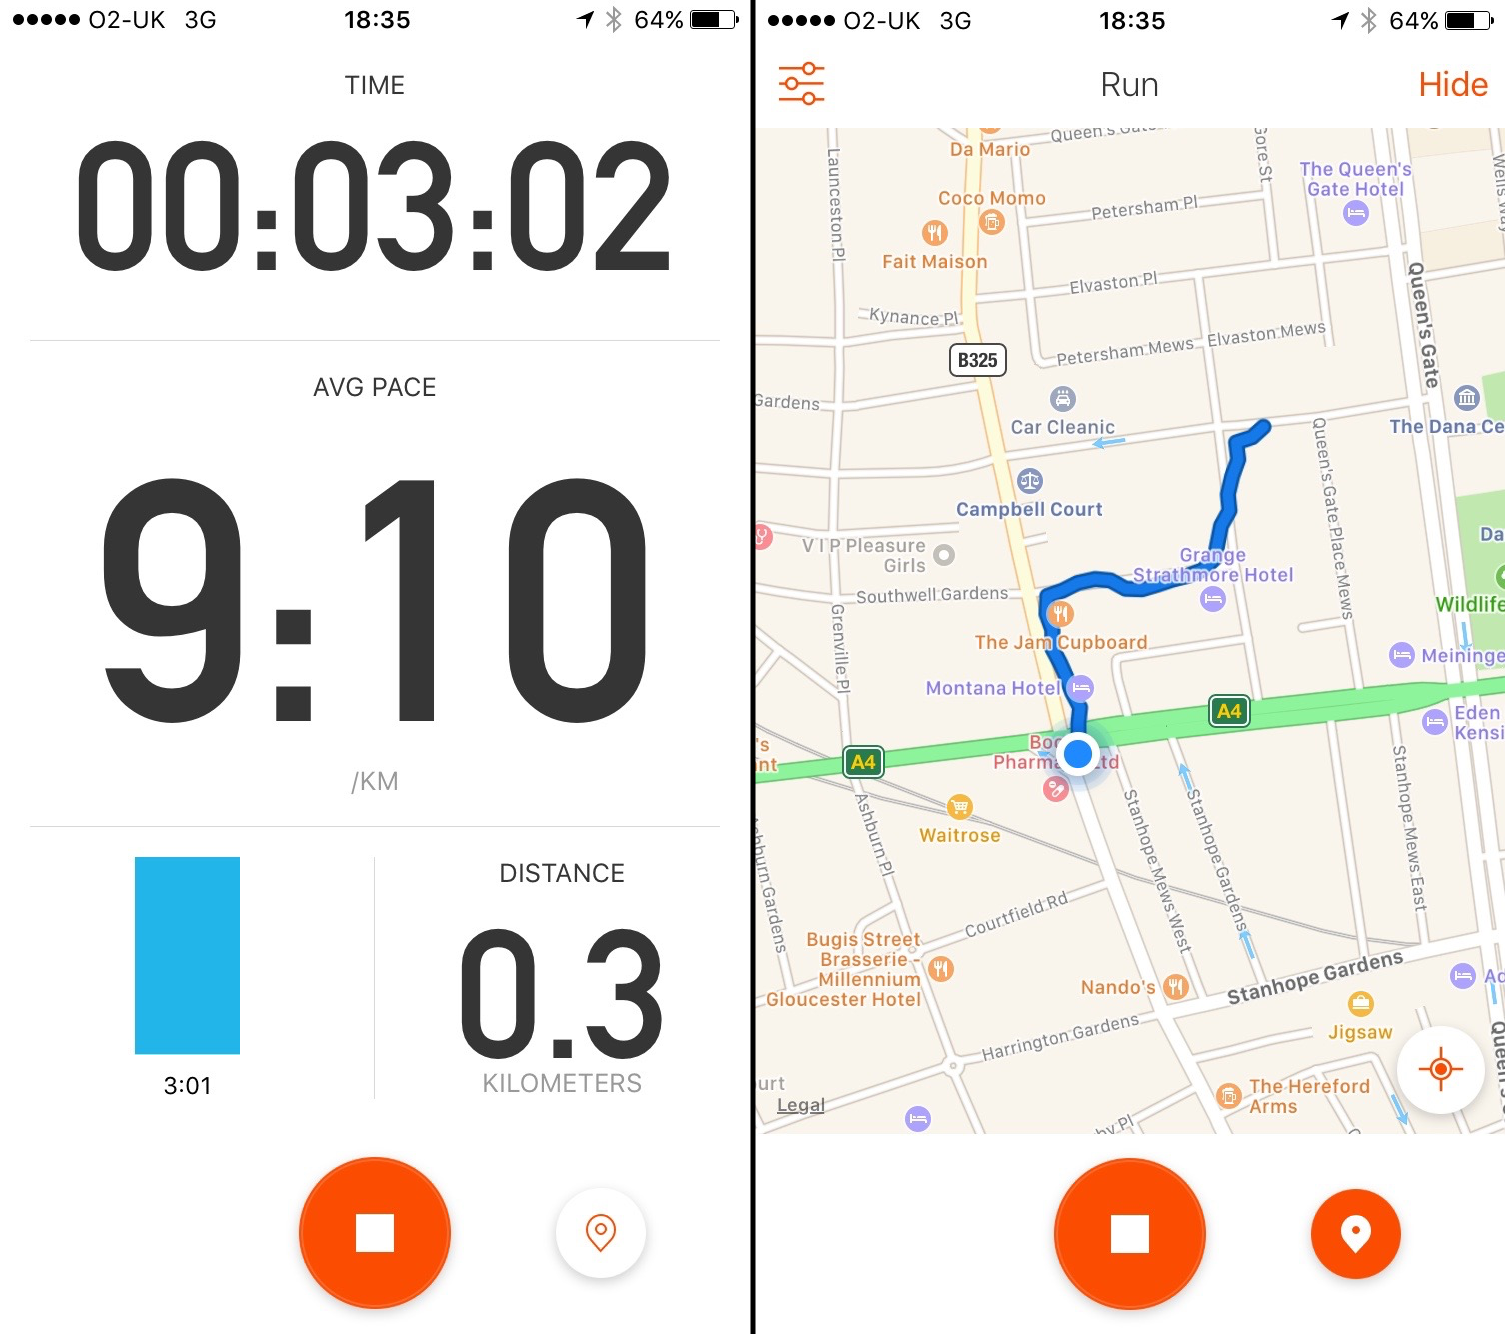
\includegraphics[width=0.7\textwidth]{strava}
  \caption{Journey view in Strava, allowing you to switch between statistics (left) or a map of your progress (right)}
  \label{fig:strava}
\end{figure}


\subsection{Let's Walk}

A lesser-known iOS fitness application is Let's Walk \cite{LetsWalkApp}. Users can record new walks and view a list of either their friends' walks or public walks nearby. The app is also focused on helping you maintain a balanced diet -- the amount of calories you consume can be added for particular meals during the day. A calorie goal per day can then be added, with the app recording how many calories were burned during a walk and updating the goal accordingly.

Let's Walk tries to emulate many of the features implemented by the more well-known apps as mentioned above, but a lot of these features seem unpolished. There is a global ranking section of the application showing which users have walked the most over the last week, month or year, however there seems to be little to do with this information other than view a leaderboard.



\subsection{Google Maps}

Although not a fitness application per say, Google Maps \cite{GoogleInc.} is one of the oldest services that provides route planning via different transport modes. The mobile app contains current information about public transport, traffic and displays well-known cycling routes on a map, however there is little in the way of customisation for walking. When entering a destination, the app generates a route but users can also choose from a few different routes on the map, with the app showing the difference in time each one would take. However, no information is given as to whether a certain route is quieter than another, for example.

\begin{figure}[hbt]
  \centering
  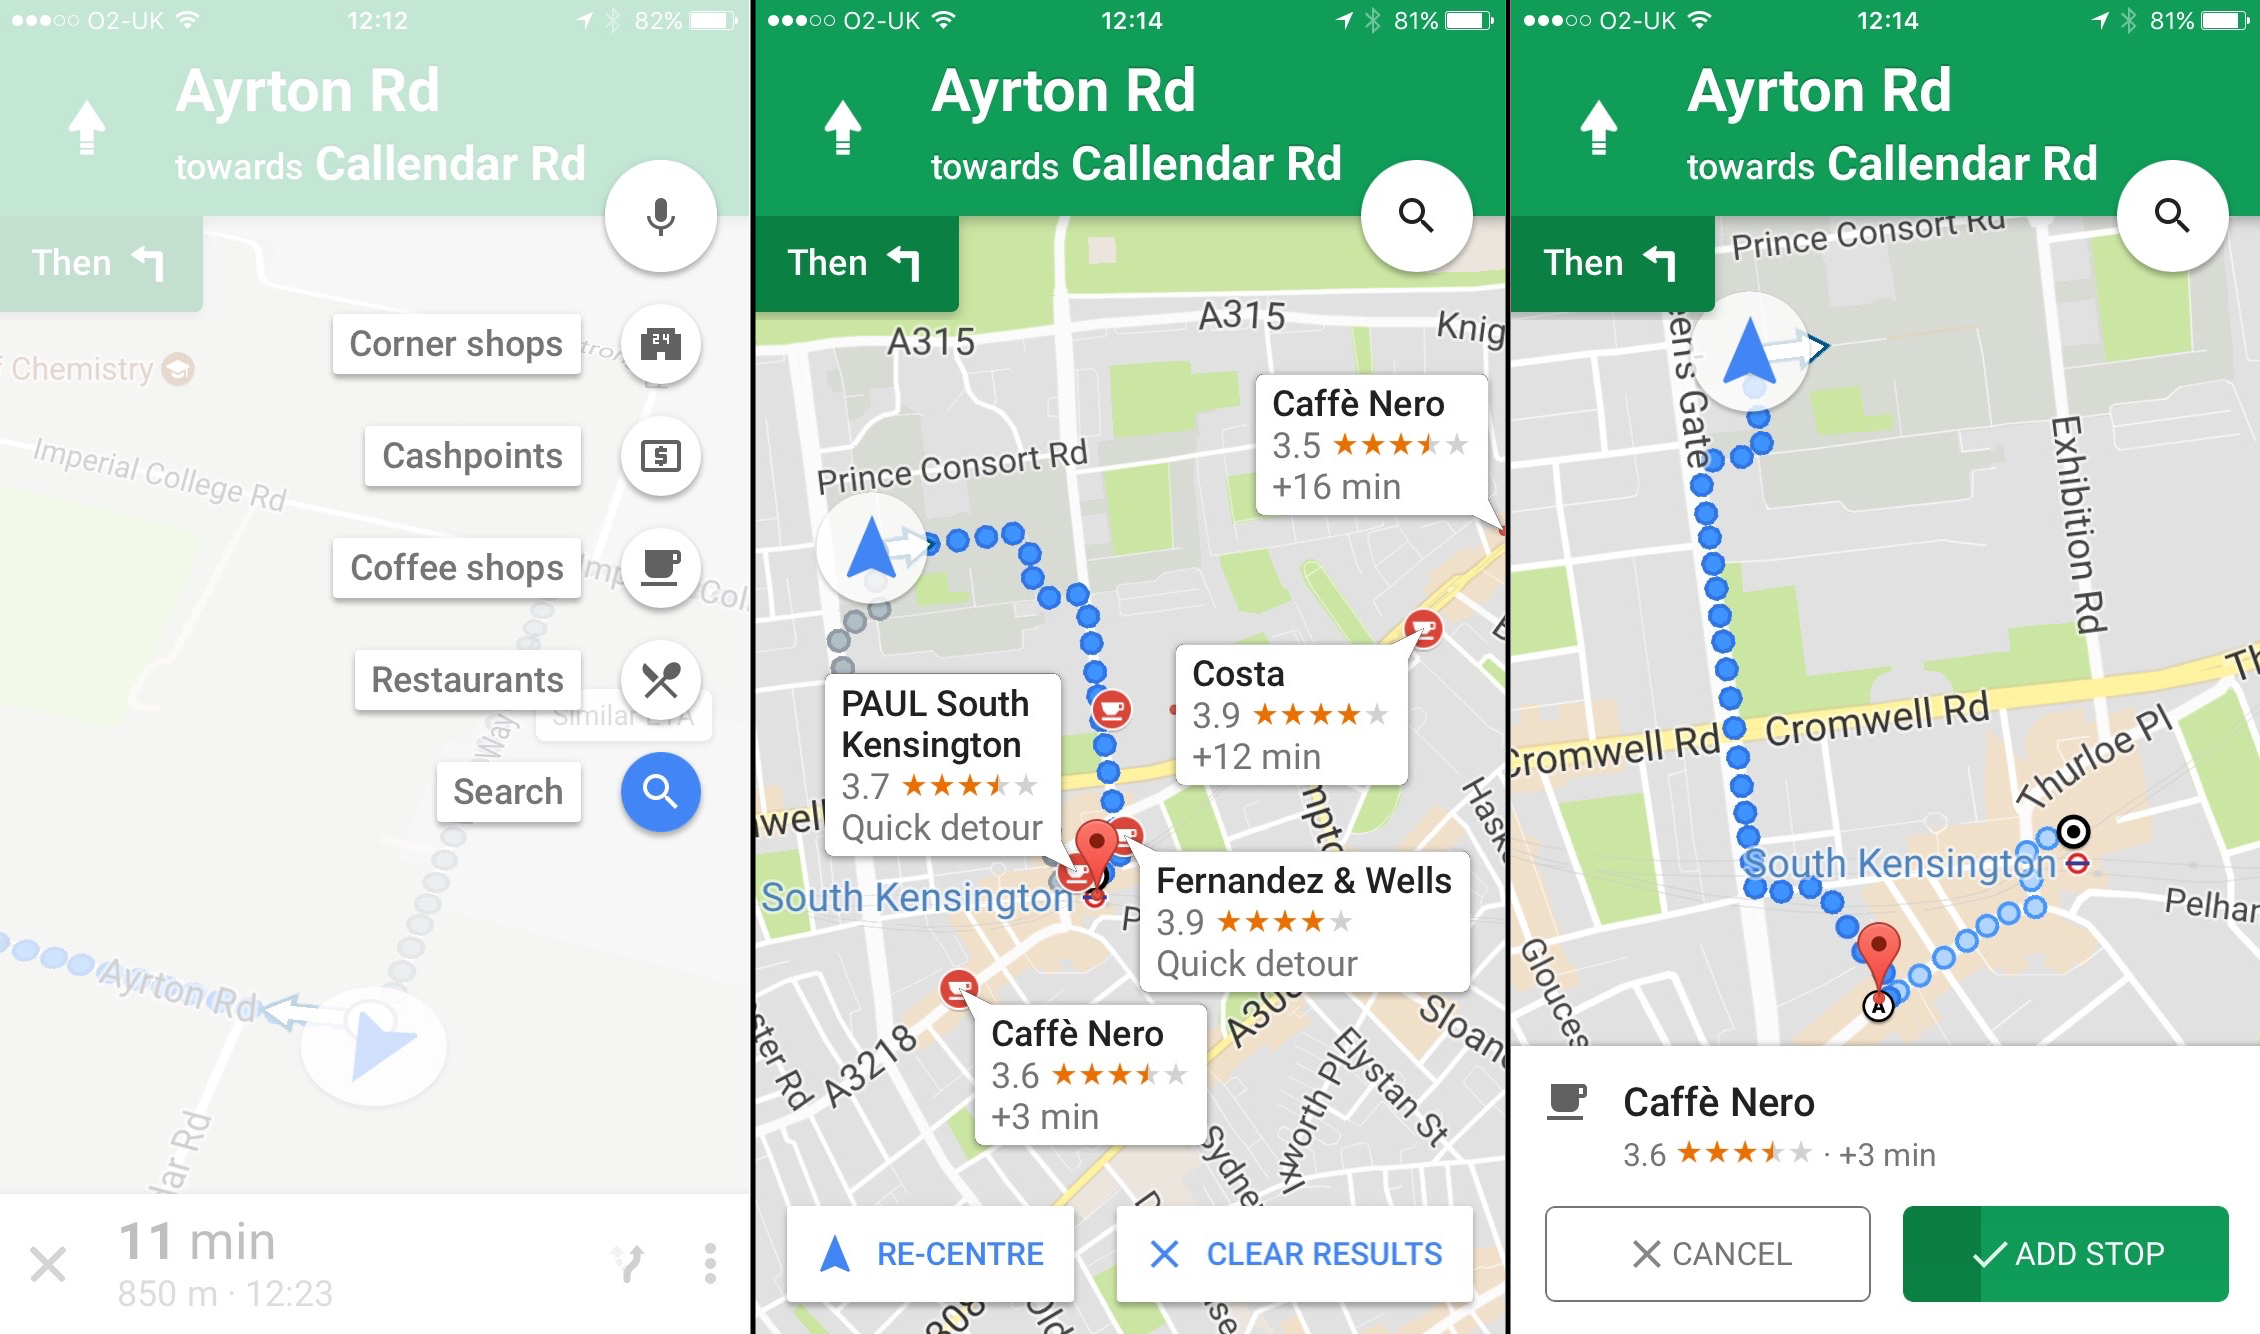
\includegraphics[width=\textwidth]{google_maps_place_search}
  \caption{Adding places along your walking route in Google Maps for iOS. A list of categories to choose from (left), then shows all the places from within a search on a map (middle). A stop can then be added and the journey will be updated (right).}
  \label{fig:google_maps_place_search}
\end{figure}


One feature of the Google Maps iOS application that is interesting to note is the ability to search for places along a route during a journey. Once a user has started a walking journey, they are able to search for places that are along the route. Google provides some categories of places to choose from, such as cashpoints and restaurants, but users can search for a specific place if they wish. The app will then display the results of the places search on the map, showing how much additional time would be added on to your journey if you were to stop at a place, if any. One or more places can then be added to your journey and the walking directions will subsequently update to include these new stops. Figure \ref{fig:google_maps_place_search} shows an example journey from Imperial College to South Kensington station. It details the full process of choosing \textit{coffee shops} as the place category, selecting a particular coffee shop on the map and the stop being added to the journey.

The places search feature is important as it is unique within any of the existing journey planner apps I have researched and it relates to one of my objectives regarding displaying points of interest when a user is on a walk (\textbf{Obj 2}). More research is conducted in Section \ref{subsection:apis} to discover what tools these applications use to implement this feature.

\subsection{Citymapper}

Originating in London, Citymapper \cite{Citymapper} has become one of the leading journey planners for major cities around the world including Paris, Barcelona, New York, Tokyo and Sydney. One of the key features of Citymapper is that different modes of transport can be combined to create a faster journey time. For example, a journey from Imperial College to Oxford Circus (as shown in Figure \ref{fig:citymapper}) could just use the Tube, but it could be faster to hire a bike and cycle to a different station and then take the Tube.

\begin{figure}[hbt]
  \centering
  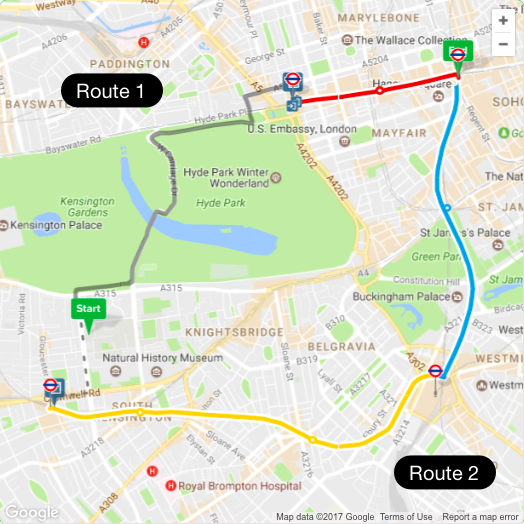
\includegraphics[width=0.7\textwidth]{citymapper}
  \caption{Two routes generated on the Citymapper website superimposed -- cycle and Tube route (Route 1) and Tube only route (Route 2)}
  \label{fig:citymapper}
\end{figure}

The walking directions in Citymapper are relatively limited. If you choose to walk on any route that you input, you are greeted with the screen shown in Figure \ref{fig:citymapper-walk}. Details such as estimated time of arrival, calorie burn and time of journey are displayed on this screen. Once you press \textit{Go}, you are transferred to the journey view, which simply tracks your location on a map and allows you to share your estimated time of arrival with others.

\begin{figure}[hbt]
  \centering
  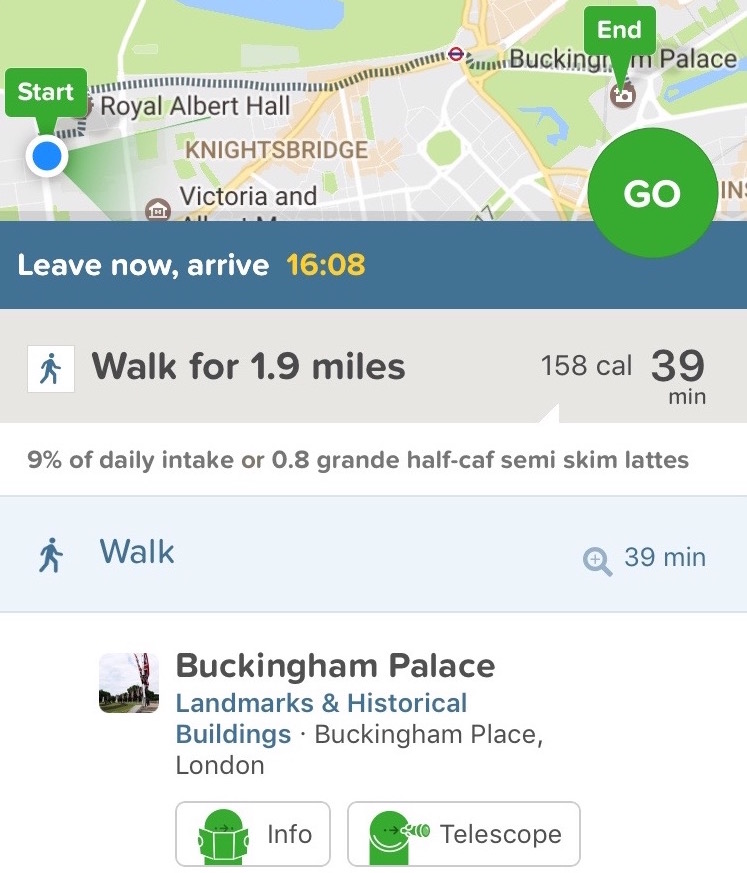
\includegraphics[width=0.55\textwidth]{citymapper_walk}
  \caption{Walking view in Citymapper}
  \label{fig:citymapper-walk}
\end{figure}

\subsection{Pok\'{e}mon Go} \label{subsection:pokemongo}

Pok\'{e}mon Go, released last July, quickly grew to become one of the most popular games of the year. Although not necessarily a walking application in the normal sense, the aim of the game is to capture virtual `creatures' called Pok\'{e}mon that appear in real world places. Thus, the game motivates you to walk more to collect more and more Pok\'{e}mon.

One of the more interesting parts of the application that is relevant to this project are the Pok\'{e}stops within the game. A Pok\'{e}stop is a location in the game where various in-game items can be collected. They are displayed on a map using blue beacons as shown in Figure \ref{fig:pokemongo}. These locations were crowdsourced by users of the game and are normally points of interest in the area such as a statue, a building or a famous plaque. Although not completely, this feature of the application does somewhat tie into my objective for helping people discover the world (\textbf{Obj 2}).

\begin{figure}[hbt]
  \centering
  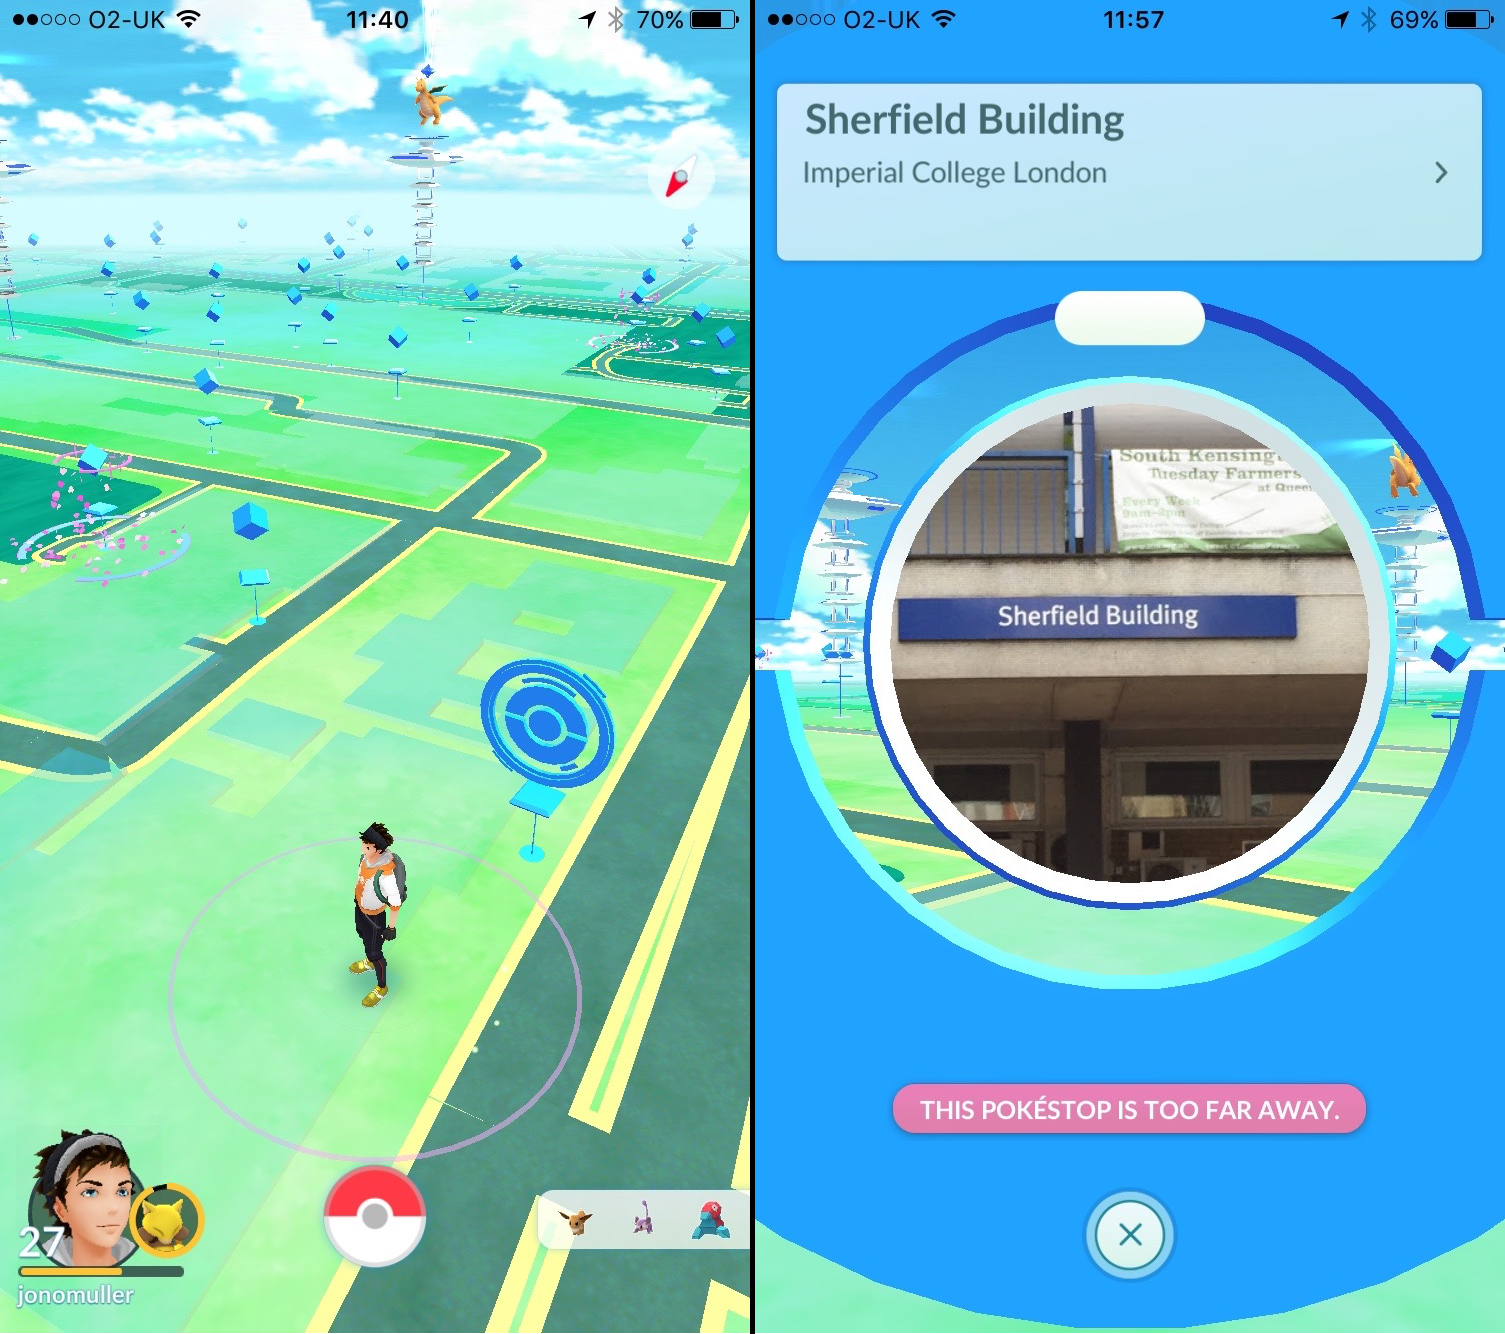
\includegraphics[width=0.7\textwidth]{pokemongo}
  \caption{Screenshots of Pok\'{e}mon Go showing Pok\'{e}stops in an area (left) and a detailed view of a Pok\'{e}stop (right)}
  \label{fig:pokemongo}
\end{figure}

\subsection{Summary}

From the subset of fitness applications that I researched in this section, it can be seen that some of the objectives I proposed in Section \ref{section:objectives} have been achieved but no single application encompasses all of my proposed objectives. I have found that it is important for this project to have a sleek design and easy-to-use interface as this is something that stood out straight away when looking at existing applications.

%\pagebreak

\section{Gamification}

% research how gamification has been used in applications, not just walking apps
% discuss how well each implementation has worked

Gamification is used in mobile applications not only for fitness but also in a wide range of areas including productivity, finance and mental health. We have seen how gamification can be used in existing fitness applications, with some apps setting challenges for users to complete within a given timeframe -- such as running a half marathon in February.

An application and website called Habitica \cite{Habitica}, labelled as a ``gamified task manager", helps motivate you to complete household tasks by unlocking features and levelling up an in-game avatar. Completing real-life tasks earns you gold for your character, which can then be redeemed for either virtual rewards such as equipment or real-life treats like watching an episode of a TV show, for example. The home page of Habitica, shown in Figure \ref{fig:habitica}, is split into columns containing your bad habits, daily tasks, to-do list and rewards. It also shows the progress of your avatar, along with what is needed to progress to the next level. This type of app helps you become more productive at home in a fun and creative way that users enjoy.

\begin{figure}[hbt]
  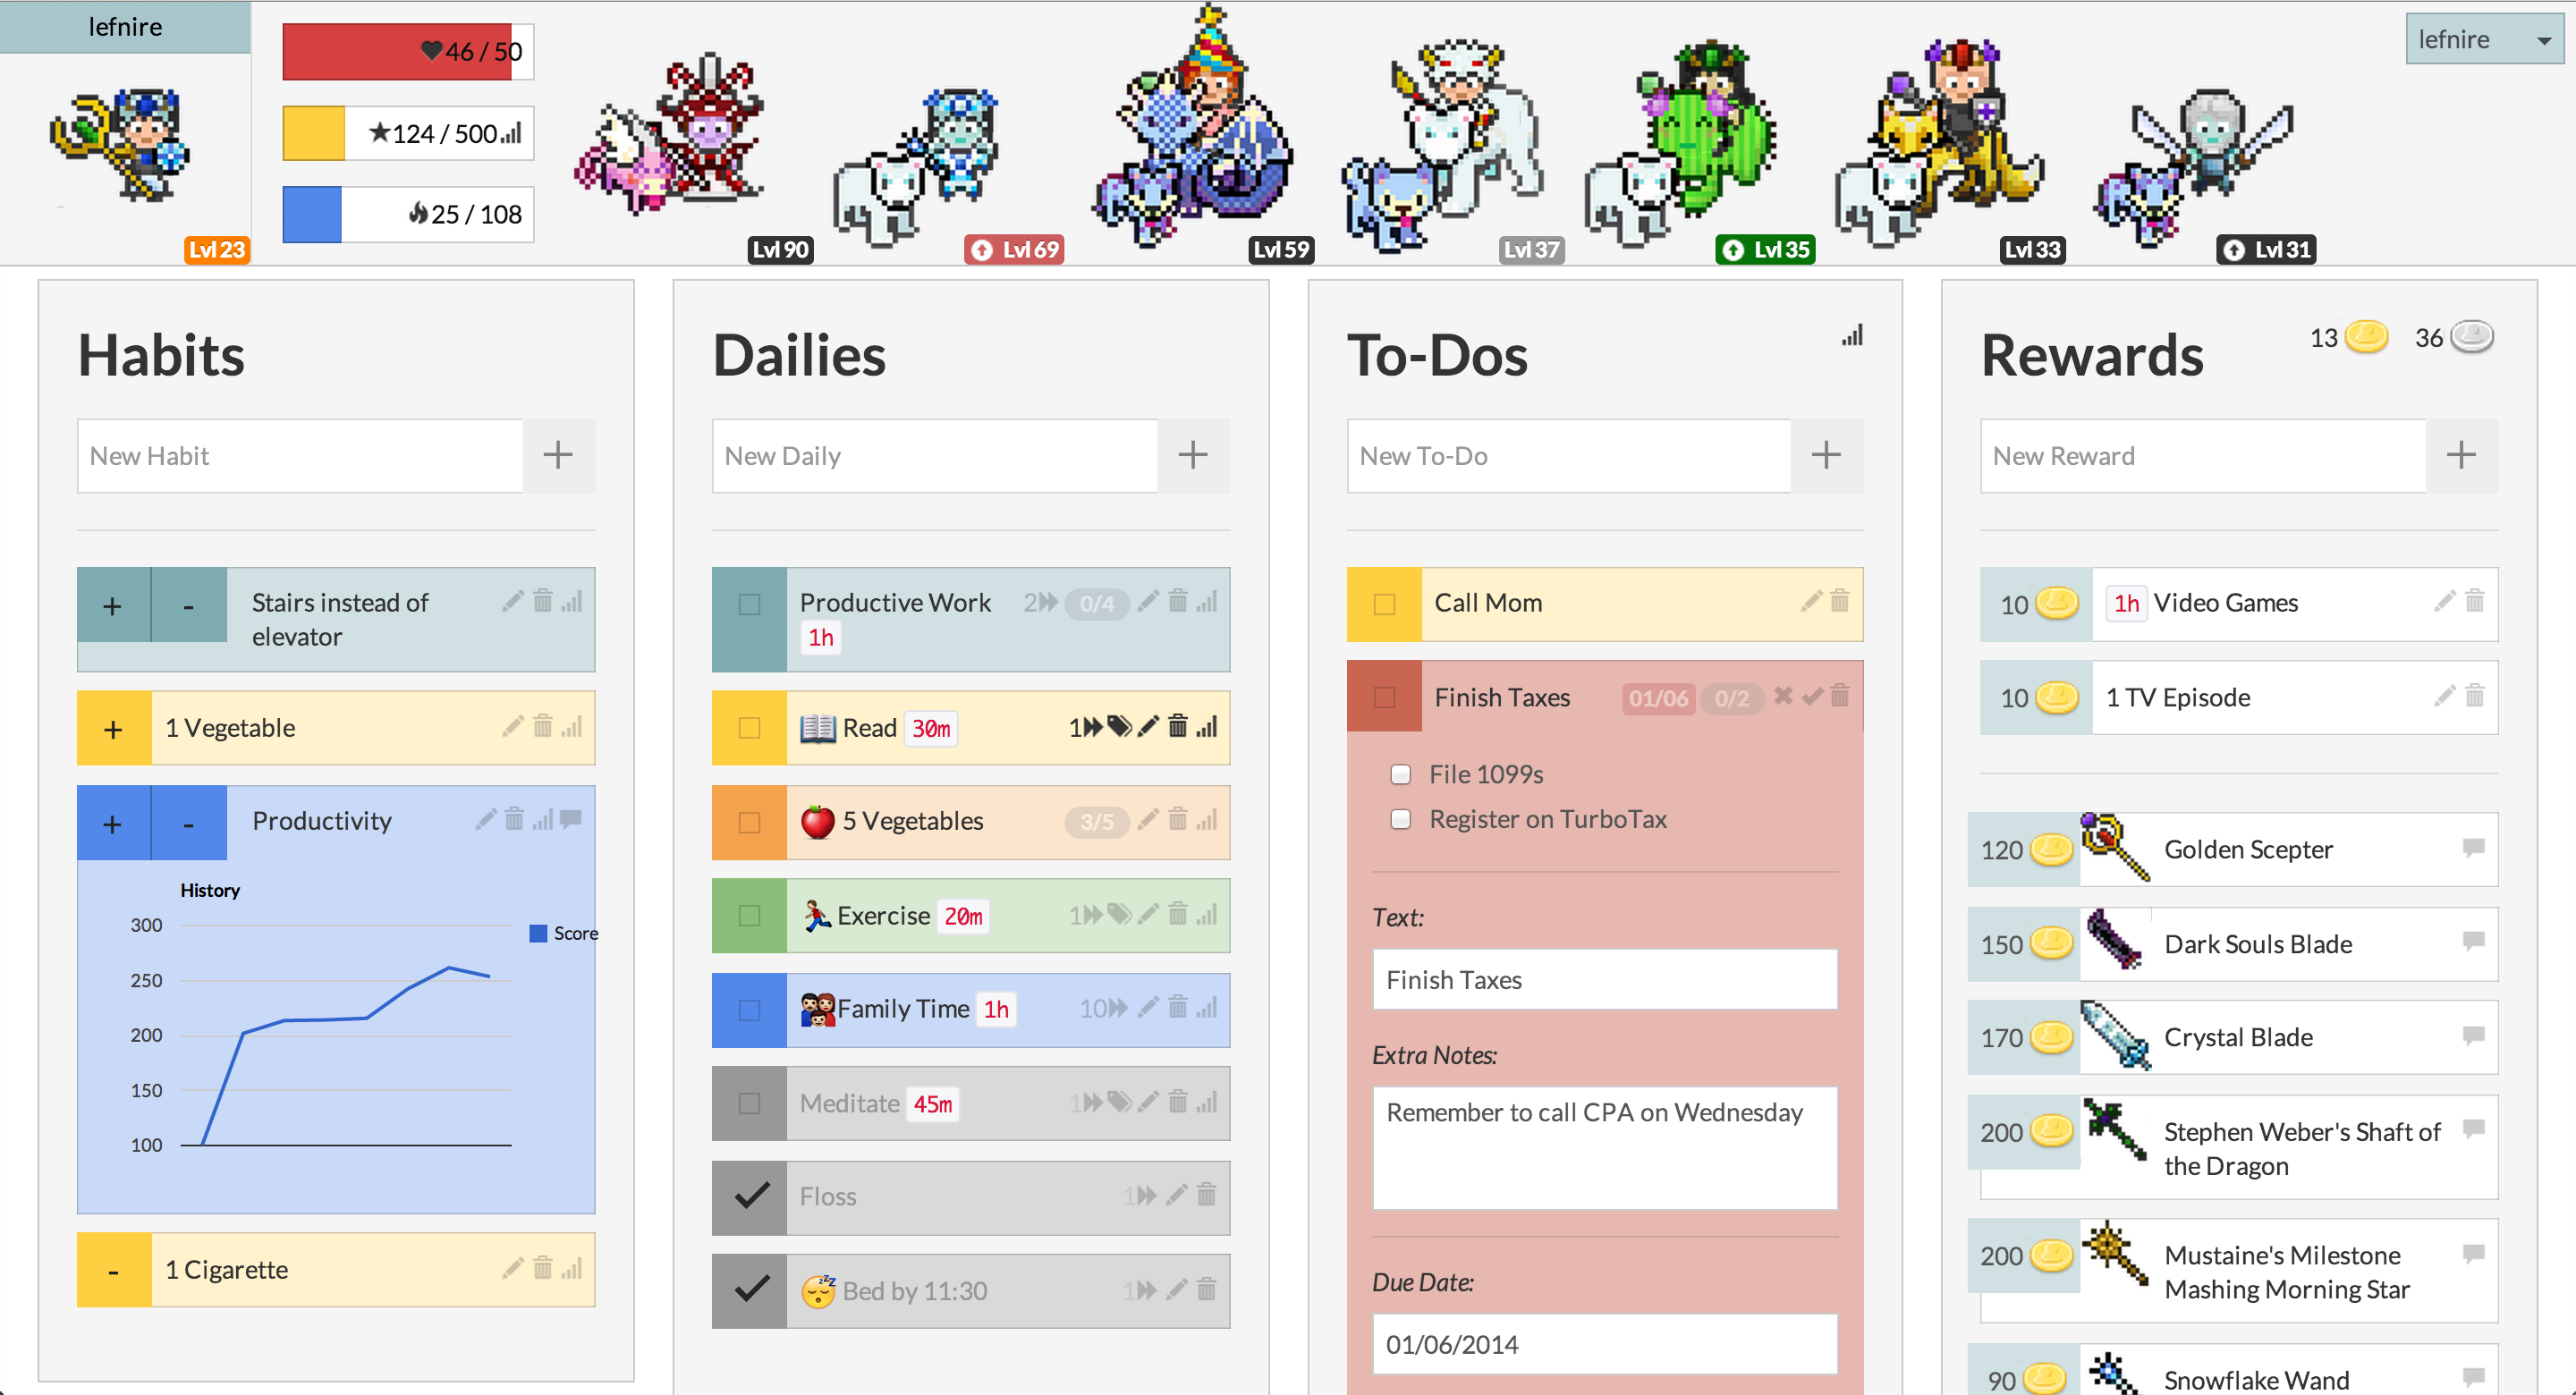
\includegraphics[width=\textwidth]{habitica}
  \caption{Home page of Habitica showing your habits, tasks and rewards as well as your avatar at the top \cite{Habiticaa}}
  \label{fig:habitica}
\end{figure}


Gamification is also used in some finance applications. Mint \cite{IntuitInc.} is an application available in America that links to your bank accounts to help you manage your bills and track how much money you spend. It shows a breakdown of what you are spending your money on and creates a budget with the option of using any left over money on goals designed to help you save money, as shown in Figure \ref{fig:mint}. You can create goals to be either a long-term one-off payment -- buying a house, for example -- or a short-term monthly payment such as a subscription service. This game mechanic of working towards a goal to help you buy something you want is extremely effective and is why gamification is so widespread.

\begin{figure}[hbt]
  \centering
  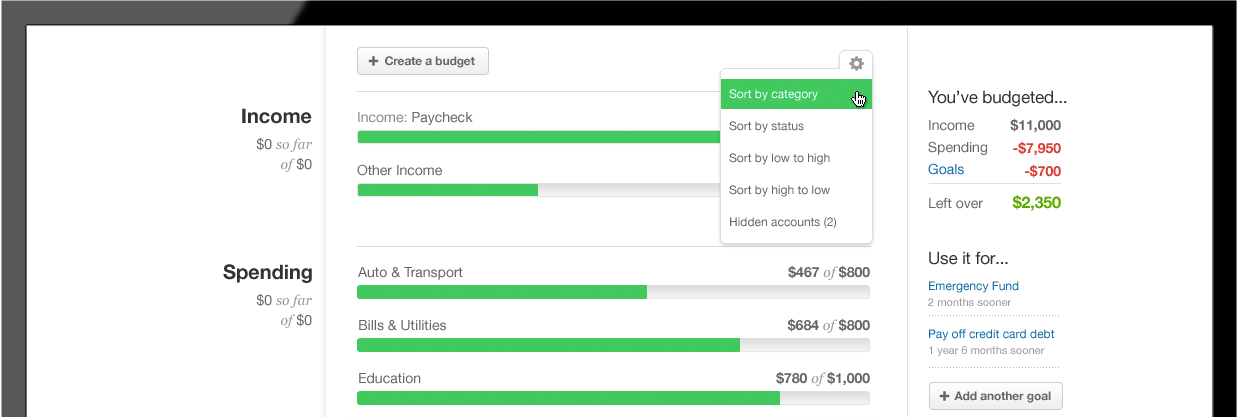
\includegraphics[width=\textwidth]{mint}
  \caption{The breakdown of spending in Mint, giving you the option to use any left over money from your budget for one or more goals \cite{IntuitInc.a}}
  \label{fig:mint}
\end{figure}

The idea of using gamification in applications is to motivate you to complete some form of task that you otherwise might not have attempted. It can make an app seem more engaging to the user, providing them with something to achieve every time they use the app. It is especially useful in fitness applications as keeping fit and staying healthy is very important, and should therefore be carefully considered for this project.

%\pagebreak

% not sure whether to include this in background or design?
% think I will include general background on technologies here, and then which ones I chose in design
\section{Technologies}

The features of existing applications are not the only important part to research -- the technologies that they use to implement these features are just as useful. This section discusses how existing applications implement certain features and which technologies integrate well with each other.

\subsection{Operating System}

Many of the applications that I have researched have been developed for iOS, the operating system running on iPhones and iPads. I have chosen to develop my application on iOS due to my previous experience with iOS app development. Another factor in this choice is that I have gained a lot of experience programming in Swift, one of the programming languages used to develop iOS apps, over the last few years. Swift is extremely readable and easy to use, which is the reason why I am choosing to use it over the other programming language available, Objective-C.

\subsection{Location Tracking}

To track the user's location within iOS, an application can use the classes from the Core Location framework \cite{AppleInc.} inbuilt into the iOS SDK (software development kit). This framework allows a developer to obtain the user's current location in the form of latitude and longitude. To keep a history of where the user has been, these coordinates could be stored in an array and updated every few seconds. This will be useful for my application to show on a map where a user has previously walked.

% section on how to track calories burned?

\subsection{Third-party APIs} \label{subsection:apis}

One of the most important application programming interfaces (APIs) to consider is which source of map to use. The majority of existing applications use Apple's maps apart from, of course, Google Maps. This is because Apple's MapKit framework \cite{AppleInc.a} is much better integrated with the Core Location framework mentioned above, making it much easier to display the user's location on MapKit than on the Google Maps SDK.

% maybe don't include
However, there are some advantages of Google Maps over Apple Maps -- one being that Google Maps tends to be more detailed than Apple Maps. An example of this is shown in Figure \ref{fig:google-apple}, where in my opinion roads are easier to see and buildings are clearly visible on Google Maps than on Apple Maps.

\begin{figure}[hbt]
  \centering
  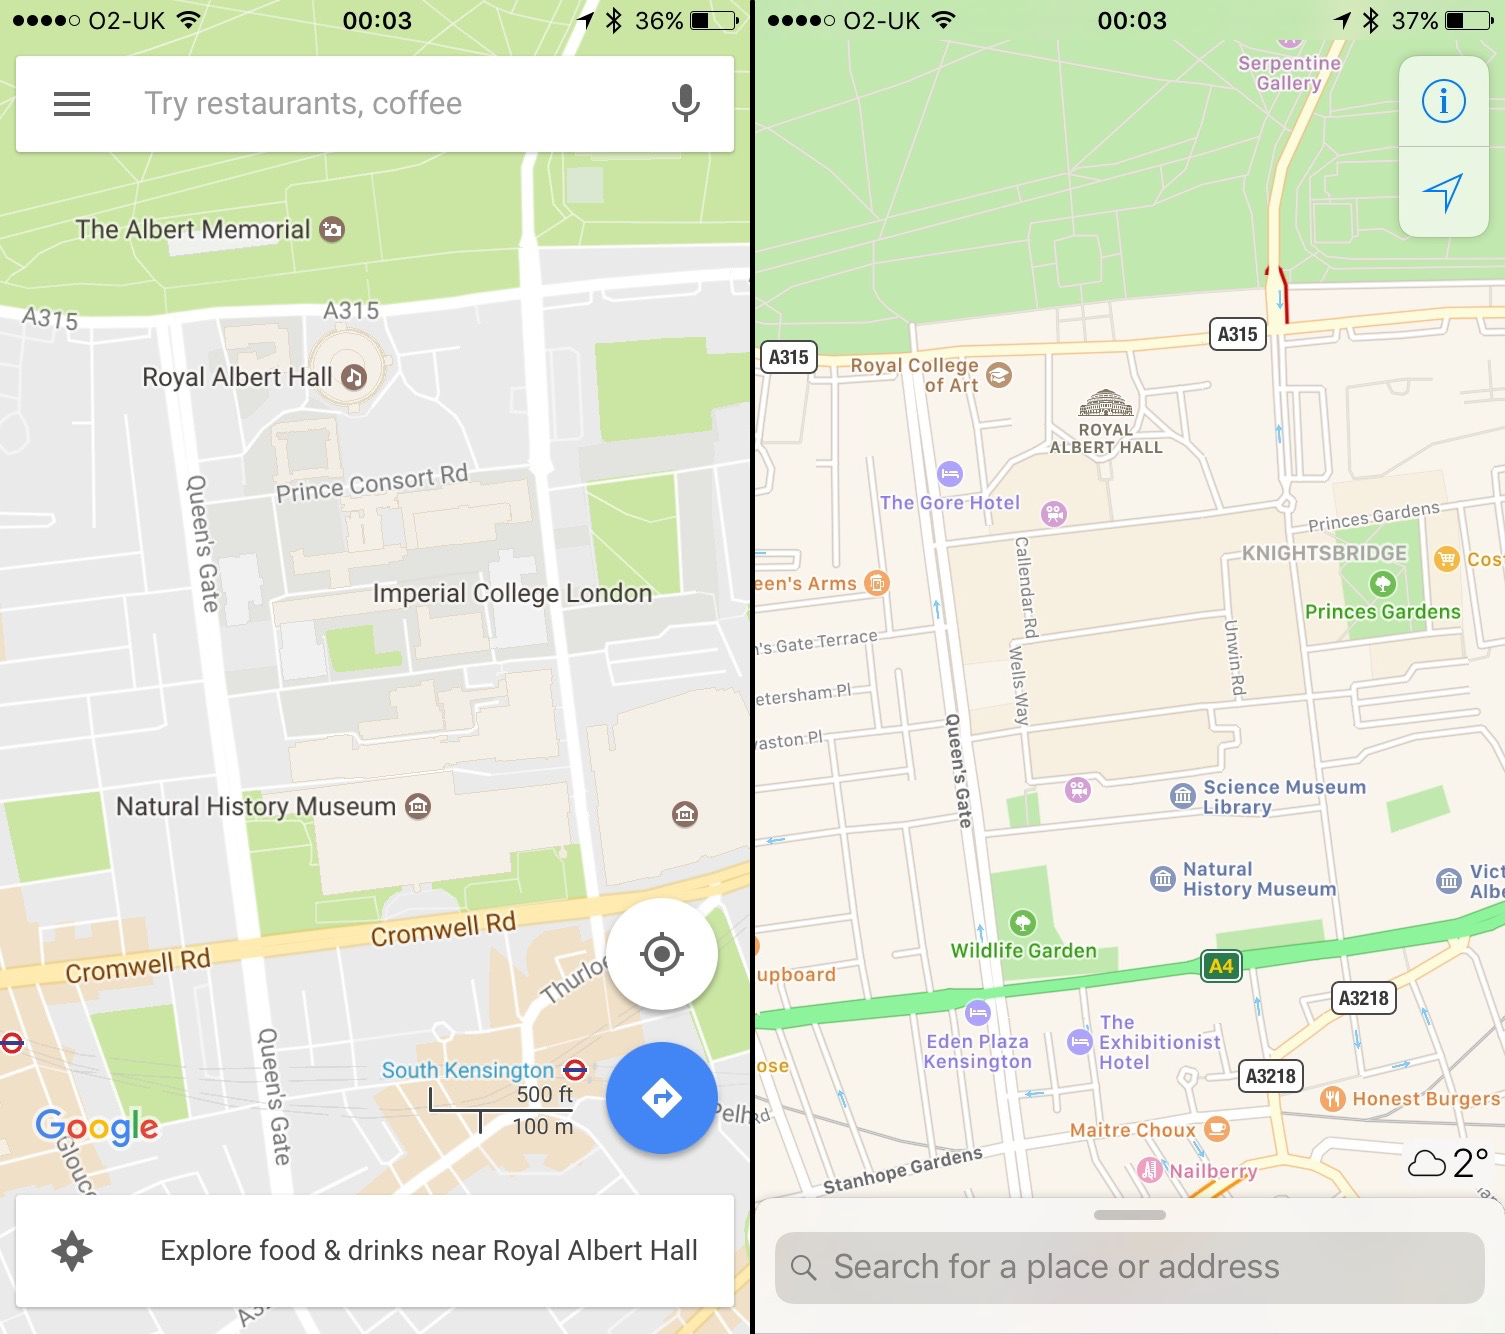
\includegraphics[width=0.7\textwidth]{google-apple}
  \caption{An example of the difference between Google Maps (left) and Apple Maps (right), showing Imperial College London}
  \label{fig:google-apple}
\end{figure}

The other API that I need to consider is one that gathers points of interest near a user's location. Google's Places API \cite{GoogleInc.b} would be a very good resource to use, allowing you to search for places by over a hundred types including \textit{point of interest}, \textit{place of worship} and \textit{museum}. The only issue with using Google Places is that you must use Google Maps to display the places on. From the Google Places Policies, \textit{``If your application displays data from the Google Places API for iOS on a map, that map must be a Google map"} \cite{GoogleInc.c}. This would mean that if I were to choose Apple Maps for the maps within the app, I would be unable to use Google Places as well.

Apple also provides an API for obtaining places called \texttt{MKLocalSearch} \cite{AppleInc.b}. To generate a list of places, you pass the \texttt{init()} method a \texttt{MKLocalSearchRequest}, which contains a string describing what type of place you would like to search for on a map. There seems to be little documentation online explaining what range of places that this API returns, which is something to consider when comparing it to other similar services.

A different option that could be used to generate points of interest around a geographical location originates from Pok\'{e}mon Go. As mentioned in Section \ref{subsection:pokemongo}, Pok\'{e}mon Go contains thousands of Pok\'{e}stops -- crowdsourced points of interest from all over the world. There exists an API \cite{Selwyn} that returns a list of Pok\'{e}stops in JSON format given a location. Each item that the API returns contains the name and location of a point of interest as shown in Listing \ref{listing:pokestop}, and so could therefore be used in this project.

\begin{listing}
  \centering
  \begin{lstlisting}[style=json]
  {
      "distance": 44, 
      "name": "Sherfield Building", 
      "bearing": 200, 
      "latitude": 51.498359, 
      "image": "http://lh3.googleusercontent.com/07q4ms3tgDKsQMy04xye
            <@\textcolor{red}{\hspace*{20pt}\_i-UiraPO3jOS18TXwKpTMecgIXm2jXByO1CAUWVW9vNgqfx12ZtjqLdZrOlfsPu}@>", 
      "guid": "2cc0f9d9c7ba49348299c15749c49ea1.16", 
      "compass": "S", 
      "longitude": -0.178544
  }, 
  \end{lstlisting}
  \caption{Example of one item returned from the Pok\'{e}stop API, with attributes including its name, latitude, longitude and distance from your location}
  \label{listing:pokestop}
\end{listing}

% add section on blue plaque API
% used based on data from research survey





